\documentclass{article}
\usepackage{graphicx}
\usepackage{geometry}
\usepackage{amsmath}
\usepackage{float}
\usepackage{xcolor}
\usepackage{listings}
\usepackage{matlab-prettifier}
\usepackage{caption}
\usepackage{subcaption}
\usepackage{xparse}
\usepackage{hyperref}
\usepackage{amssymb}
\usepackage{verbatim}
\usepackage{fancyhdr}
\pagestyle{fancy}
\usepackage{xspace}
\cfoot{}
\lfoot{Università degli Studi di Padova, Reti di Calcolatori 1, AA 2022-2023}
\rfoot{\thepage}

\newcommand{\Rcerchio}{\textregistered\xspace}

\title{Homework 2\\\textbf{Metriche di rete con comando \texttt{ping}}}
\author{Giacomo Calabria - 2007964}
\date{\today}

\begin{document}
    \maketitle
    \section{Introduction}
    L'obiettivo di questo Homework è quello di produrre un programma che effettui una semplice tecnica di codifica basata sulla DCT.\\\\
Il codice fornito è stato scritto nell'ambiente di programmazione MATLAB\Rcerchio in quanto esso dispone della libreria \textit{Image Processing Toolbox} che offre molti strumenti per manipolare ed elaborare in modo semplice le immagini, tra cui comprese la funzione DCT. Inoltre, la possibilità di visualizzare immagini e manipolarle in modo facile e intuitivo è estremamente utile per analizzare e valutare la qualità della codifica effettuata.\\\\
Per eseguire il codice, è necessario salvare l'immagine da elaborare nella stessa cartella del file MATLAB, quindi aprire il file e premere il tasto "Run" o digitare il comando \texttt{"run Project1.m"} nella finestra della console di MATLAB.\\\\
Il codice utilizza alcune funzioni matematiche standard di MATLAB per calcolare il MSE e il PSNR e tracciare le curve del PSNR in funzione di R. E richiede la libreria \textit{Image Processing Toolbox} per gestire l'elaborazione di immagini e in particolare la funzione DCT.\\\\
Il codice richiede l'impostazione di alcuni parametri di input:
\begin{itemize}
    \item Il path/nome del file
    \item Dimensione dei blocchi $N$
    \item La percentuale $R$ di coefficienti DCT da mettere a zero
\end{itemize}
Questi parametri possono essere modificati all'interno del file MATLAB\Rcerchio.

    
    \section{Stima del numero di link attraversati}\label{ch:link}
    Nell'header del protocollo IP, il \textit{Time-To-Live} (TTL) è un campo che viene impostato dal mittente e decrementato di una unità ogni qual volta il pacchetto viene inoltrato da un nodo intermedio. Questo campo ha lo scopo di evitare che i pacchetti rimangano intrappolati indefinitamente nella rete. Quando un nodo riceve un pacchetto con un TTL di 1, se non è il destinatario finale, scarta il pacchetto e invia un messaggio di errore all'applicazione mittente. Pertanto, il TTL determina il numero massimo di link che il pacchetto può attraversare prima di raggiungere la sua destinazione.\\\\
Per stimare il numero di link attraversati da un pacchetto, abbiamo sfruttando l'opzione del comando \texttt{ping} che permette di variare il campo TTL \texttt{[ -t ttl]}. Specificando il valore iniziale del TTL da utilizzare durante l'invio dei pacchetti, abbiamo gradualmente incrementato il valore del TTL finchè non abbiamo ottenuto una connessione senza errore, indicando che il pacchetto è riuscito a raggiungere la destinazione. \\\\
Abbiamo creato uno script bash "ping\_ttl.sh" che automatizza questo processo e ci permette di determinare il valore minimo di TTL. Per eseguirlo è necessario inserire il comando da terminale: \texttt{sudo bash ./ping\_ttl.sh}\\\\
Lo script ha prodotto il seguente output:
\begin{verbatim}
sudo ping -c 2 -t 4 lon.speedtest.clouvider.net
sudo ping -c 2 -t 5 lon.speedtest.clouvider.net
[...]
sudo ping -c 2 -t 10 lon.speedtest.clouvider.net
sudo ping -c 2 -t 11 lon.speedtest.clouvider.net

E' necessario attraversare: n = 11 link per raggiungere la destinazione

traceroute to lon.speedtest.clouvider.net (5.180.211.133), 30 hops max, 60 byte...
 1  _gateway (192.168.5.253)  0.585 ms  0.559 ms  0.556 ms
 2  10.255.250.1 (10.255.250.1)  0.727 ms  0.812 ms  0.960 ms
 3  pdma-s25.wind.it (151.6.140.15)  8.553 ms  8.550 ms  8.547 ms
 4  151.6.140.18 (151.6.140.18)  3.926 ms  3.924 ms  4.062 ms
 5  151.6.2.10 (151.6.2.10)  8.818 ms  8.813 ms  8.811 ms
 6  151.7.112.69 (151.7.112.69)  15.662 ms  12.502 ms  12.494 ms
 7  linx-lon1.eq-ld8.peering.clouvider.net (195.66.225.184)  32.714 ms  44.599 ...
 8  10.1.10.65 (10.1.10.65)  32.670 ms  32.667 ms  32.831 ms
 9  185.245.80.44 (185.245.80.44)  32.607 ms  32.605 ms  32.602 ms
10  185.245.80.45 (185.245.80.45)  37.011 ms  37.008 ms  37.007 ms
11  5.180.211.133 (5.180.211.133)  31.788 ms  31.785 ms  31.497 ms
\end{verbatim}
Abbiamo avviato i test con un valore iniziale di TTL pari a 4, poiché i primi nodi della rete sono dedicati all'uscita dal modem e quindi non ha senso testarli. Successivamente, abbiamo confrontato i risultati ottenuti utilizzando lo strumento di tracciamento del percorso \texttt{traceroute}. In entrambi i test, abbiamo osservato che il numero di link attraversati era di 11.\\\\
Tuttavia, è importante notare che il numero di link attraversati ottenuto tramite il decremento del TTL o mediante l'utilizzo di \texttt{traceroute} non include il percorso di ritorno. Pertanto, per ottenere il numero totale di link $n$ attraversati durante il percorso di andata e ritorno, dobbiamo considerare il doppio del valore ottenuto tramite TTL o \texttt{traceroute}.
    \clearpage

    \section{Andamento di RTT}
    Per valutare l'andamento dell'RTT minimo, medio, massimo e della deviazione standard in funzione della dimensione del pacchetto abbiamo creato uno script bash "ping\_rtt.sh". Questo script automatizza il processo di esecuzione del comando \texttt{ping} con diverse dimensioni del pacchetto e raccoglie i valori di RTT corrispondenti.\\\\
Lo script utilizza un ciclo \texttt{for} per iterare attraverso una serie di dimensioni del pacchetto. Per ogni dimensione del pacchetto, esegue il comando ping specificando il numero di pacchetti da inviare e la dimensione del payload del pacchetto.\\ Successivamente, estrae l'ultima linea di output del comando ping, che contiene i valori di RTT minimo, medio, massimo e deviazione standard. Questi valori vengono salvati in un file di testo in un formato conveniente per l'acquisizione dei dati da parte di MATLAB \Rcerchio.\\\\
Nel test, abbiamo scelto di inviare per ogni dimensione del pacchetto $K=100$ pacchetti per avere una valutazione migliore delle statistiche dell' RTT. La dimensione dei pacchetti è variabile da 10 a 1472 byte con passi di 1 byte. Questa scelta ci consente di ottenere una rappresentazione dettagliata dell'andamento dell'RTT in base alla dimensione del pacchetto.\\\\
Si è scritto un programma MATLAB \Rcerchio che legge i dati dal file e genera un semplice grafico dei valori di RTT in funzione della dimensione del pacchetto. Abbiamo riportato in Figura \ref{fig:risRTT} i risultati.
\section{Stima di \textit{R} e \textit{R-bottleneck}}
Sappiamo che generalmente l'RTT aumenta con la lunghezza dei pacchetti, nella pratica questa regolazione può essere influenzata dalla variabilità del ritardo di accodamento. Considerando il valore minimo dell'RTT possiamo mitigare l'effetto dei ritardi di accodamento, misurato su una serie di trasmissioni con pacchetti di dimensione costante. Infatti si ipotizza che prima o poi il pacchetto possa trovare tutte le code vuote ad ogni nodo. In formule, assumeremo che, eseguendo un numero $K$ sufficientemente grande di volte il \texttt{ping} con $L$ costante, si abbia:
\begin{equation}
    RTT_{\min}(L)\approx aL+T
\end{equation}
In effetti, come osservato dalla Figura \ref{fig:risR} è evidente che l'andamento del minimo dell'RTT per ogni valore di $L$ è stato ben approssimato linearmente da una retta. La linearità dell'andamento del minimo dell'RTT implica che all'aumentare della dimensione dei pacchetti, il tempo di trasmissione minimo aumenta proporzionalmente.
\begin{figure}[H]
    \centering
    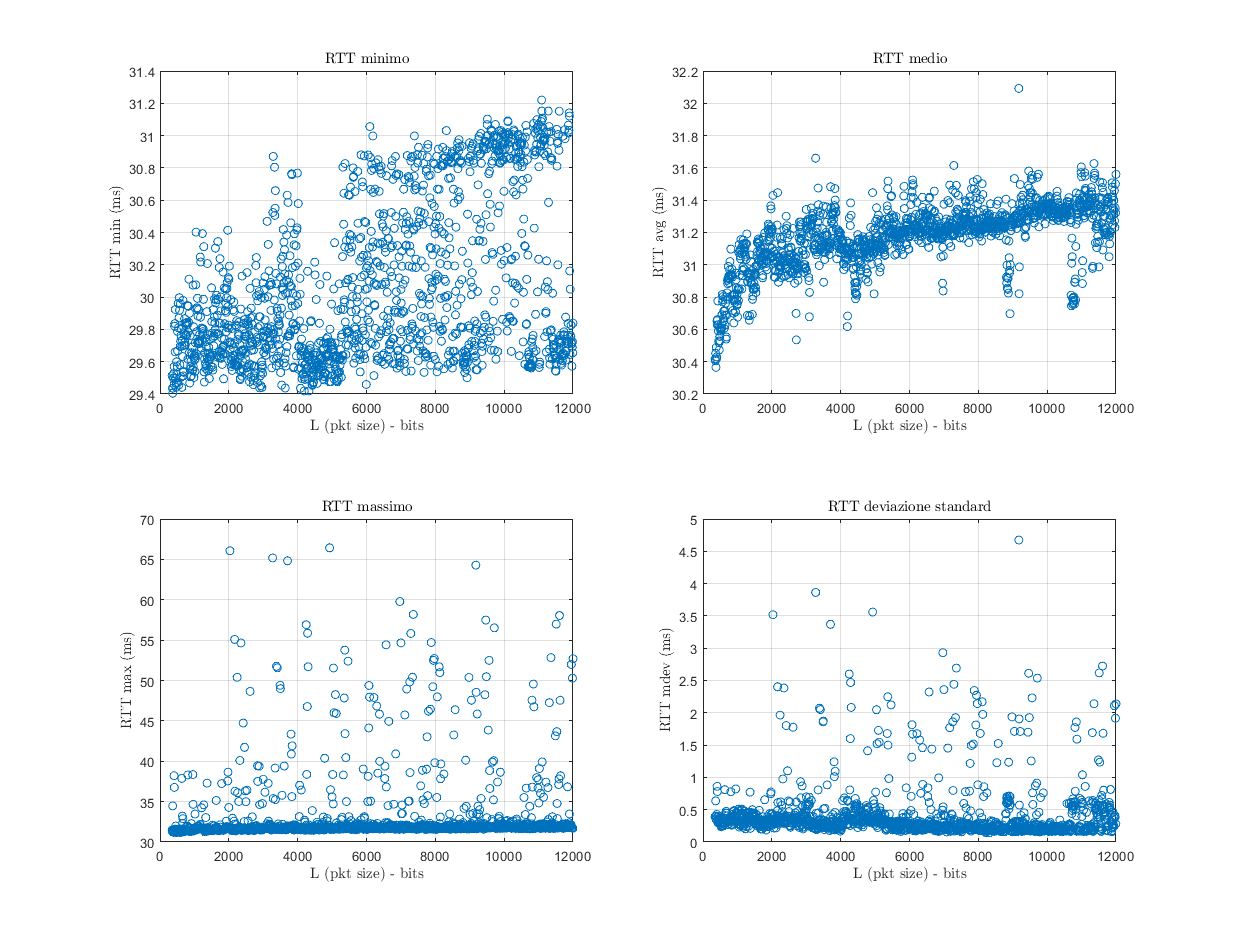
\includegraphics[width=\linewidth]{rtt all.png}
    \caption{Statistiche dell'RTT in funzione della dimensione del pacchetto}
    \label{fig:risRTT}
\end{figure}
\begin{figure}[H]
    \centering
    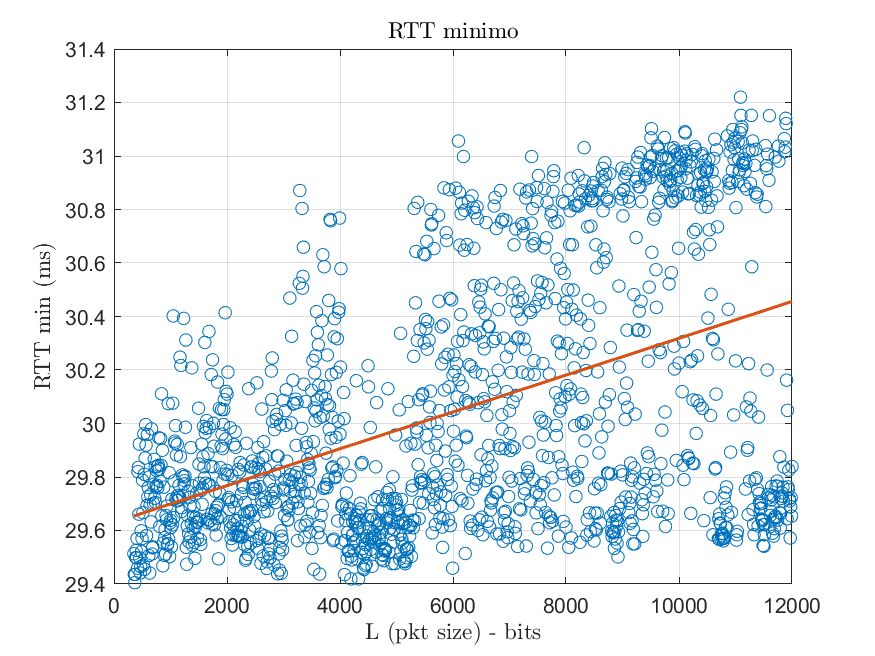
\includegraphics[width=\linewidth]{rtt fit.png}
    \caption{Statistiche dell'RTT minimo in funzione della dimensione del pacchetto con curva di andamento}
    \label{fig:risR}
\end{figure}
Stimando la pendenza della retta che approssima l'andamento del minimo dell'RTT in funzione delle dimensioni dei pacchetti, possiamo ottenere una stima del coefficiente $a$. Questo coefficiente ci fornisce informazioni utili per valutare il throughput della rete in due diverse ipotesi:
\begin{itemize}
    \item Se tutti i link (andata e ritorno) hanno throughput uguali ad un certo valore $R$, si ottiene
    \begin{equation}
        R=\frac n a
    \end{equation}
    \item Se invece esiste un link con un throughput molto minore di tutti gli altri (detto \textit{bottleneck}), e supponendo che tale throughput sia lo stesso all’andata ed al ritorno si ha:
    \begin{equation}
        R_{\text{bottleneck}}\approx \frac 2 a
    \end{equation}
\end{itemize}
\clearpage
È importante sottolineare che queste stime sono basate sulle ipotesi semplificate sull'omogeneità dei link e sulla simmetria del throughput nel caso del bottleneck. Sappiamo dalle stime fatte al punto \ref{ch:link} che il server \texttt{"lon.speedtest.clouvider.net"} ha $n=11*2=22$ pertanto otteniamo:
\begin{equation*}
    a=6.8818\cdot10^{-5}\quad R=319.6849\text{ kbps}\quad R_{\text{bottleneck}}=29.0623\text{ kbps}
\end{equation*}
\section{Conclusioni}
Attraverso l'utilizzo dell' applicazione \texttt{ping} e l'analisi dei valori di RTT siamo stati in grado di apprezzare l'andamento dell'RTT in relazione alla dimensione dei pacchetti, riusciendo a mitigare l'impatto dei ritardi di accodamento sulla misurazione.\\\\
Abbiamo osservato che, sebbene l'RTT tendenzialmente cresca con la lunghezza dei pacchetti, questa relazione può essere influenzata dalla variabilità del ritardo di accodamento. Tuttavia, abbiamo dimostrato che considerando il valore minimo di RTT misurato su una serie di trasmissioni con pacchetti di dimensione costante, possiamo mitigare l'impatto dei ritardi di accodamento.\\\\
Abbiamo ripetuto l'esperimento anche con altri server: ottenendo prestazioni peggiori con server più lontani geograficamente.
\end{document}
